
\section{Measurements}
\label{sec:meas}

This work is focused on measuring turbulence from moored ADVs that are equipped with inertial motion sensors (IMU). The ADVs utilized for these measurements were all equipped with Microstrain 3DM-GX3-25 IMU sensors that captured all 6 components of the ADV motion (3 components of angular rotation and 3 components of linear acceleration), as well the orientation of the ADV pressure-case. The sampling of the motion sensor is tightly synchronized with the ADV measurements. The IMU measures its motion at 1kHz and uses internal signal integration (Kalman filtering) to output the motion signals at the same sample rate as the ADV's velocity measurements. This reduces aliasing of the IMU's motion measurements above the ADV's sample-rate \citep[]{3DM-GX3_coning_sculling}.

\subsection{Measurements}

This work utilizes data from two distinct mooring systems to demonstrate the advantages and limitations of each platform. Both mooring systems were deployed in Admiralty Inlet, Washington, approximately 500 meters (m) WSW of Admiralty Head--Fort Casey State Park--in 60 m of water depth at latitude 48.153 north and longitude 122.687 west (Figure \ref{fig:map}). The site is approximately 6 kilometers (km) east of Port Townsend, and 1 km north of the Port Townsend -- Coupeville ferry route.  
Admiralty inlet is the largest waterway connecting Puget Sound to the Strait of Juan de Fuca, and it possesses a large semi-diurnal tidal flow.

\begin{figure}[t]
  \centering
  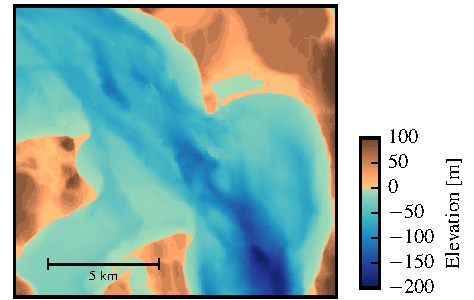
\includegraphics[width=3.4in]{map04.pdf}
  \caption{Bathymetry of Admiralty Inlet at Admiralty Head.}
  \label{fig:map}
\end{figure}

\subsubsection{Tidal Turbulence Mooring (TTM)}

The `Tidal Turbulence Mooring' (TTM) is a simple mooring system with a `strongback fin' suspended between a steel clump-weight anchor weighing 1200 kilograms (kg, dry) and a 0.93 m-diameter spherical steel buoy with a buoyancy of 320 kg . The ADV pressure cases were clamped to one side of a `strongback' fin and the ADV sensor head was positioned 10cm in front of the fin's leading edge (Figure \ref{fig:ttm:diagram}). The leading edge of the fin is fastened inline with the mooring line. This configuration  was designed to work similar to a weather-vane, such that the drag on the fin held the ADV head upstream of the mooring components.  This work utilizes data from two TTM deployments. 

The first was in June of 2012 at 48.15285 north, 122.68581 west, near Admiralty Head in Puget Sound, Washington (USA). The mooring was in the water from 17:30 on the 12th until 14:30 on the 14th (local time). Two Nortek ADVs were clamped to either side of the fin such that the axis of their cylindrical pressure-cases were parallel with the leading edge of the strongback. Only one of these ADVs was equipped with an integrated IMU. This TTM also had an upward-looking acoustic Doppler profiler mounted on the mooring anchor.

Periods of time during which this mooring interfered with a beam of the Doppler profiler were identified by inspection of the profiler's acoustic amplitude signal. Periods during which one beam of the profiler had $>5\%$ higher acoustic amplitude than the other beams were flagged as `contaminated' and excluded from averaging.  5-minute averages in which more than 50\% of the data was contaminated in this way are not shown.

The second TTM deployment was in 2014 from 06:00 on June 17 to 05:00 on June 19. The mooring was positioned at 48.15327 north, 122.68654 west.  Two Nortek ADV-IMUs were mounted on this TTM. In this case the pressure-cases and ADV heads were inclined at an angle of 18$^\circ$ to the leading edge of the fin to account for mooring blow-down during strong currents (Figure \ref{fig:ttm:photo}). This change reduced vibrational motion believed to be associated with vortex shedding from the ADV pressure cases when they are oriented cross-wise to the flow (as in the June 2012 deployment).

\begin{figure}[t]
  \centering
  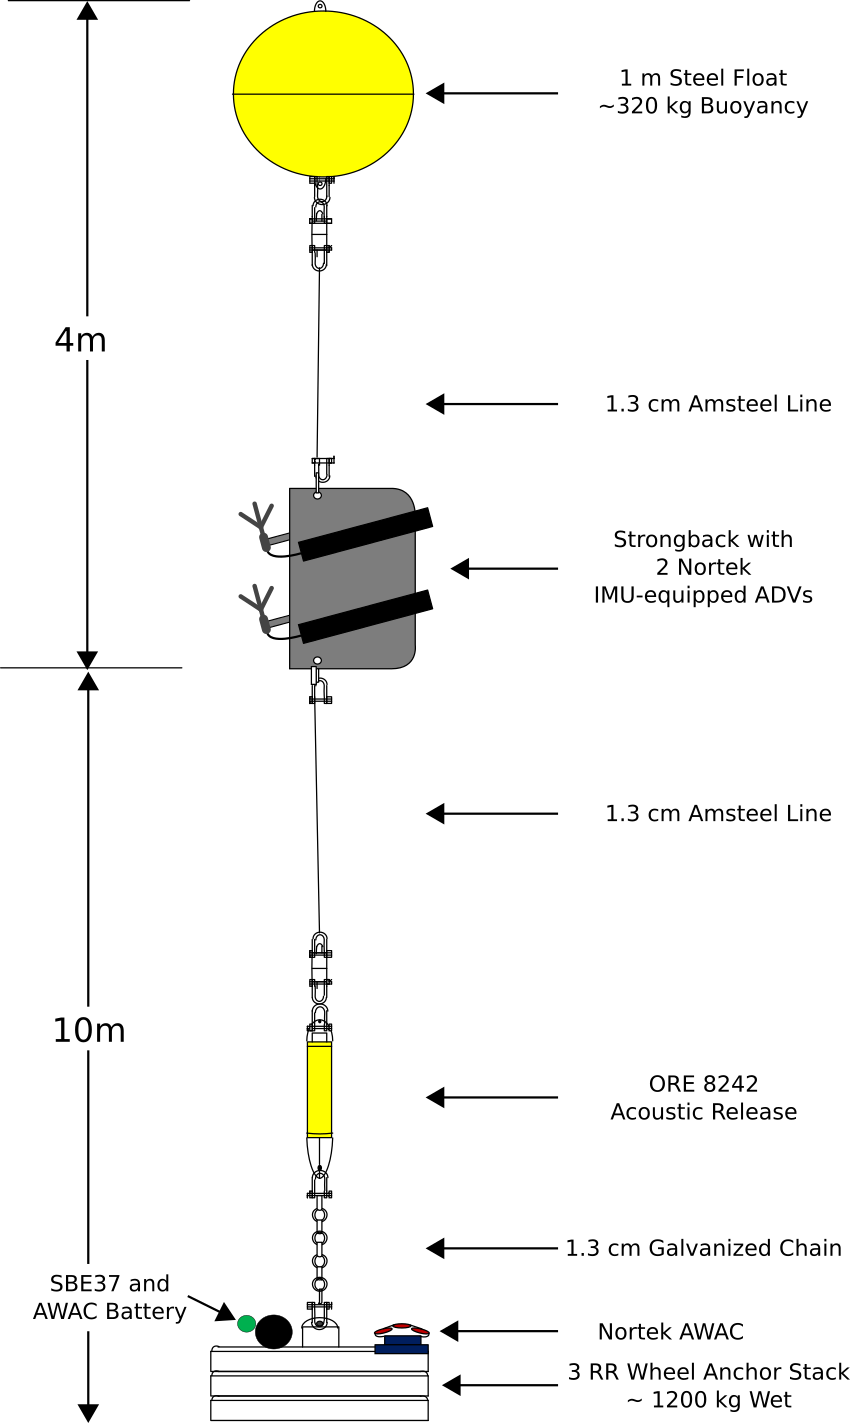
\includegraphics[width=2.4in]{ttm04b}
  \caption{Schematic diagram of the TTM, not to scale.}
  \label{fig:ttm:diagram}
\end{figure}

\begin{figure}[t]
  \centering
  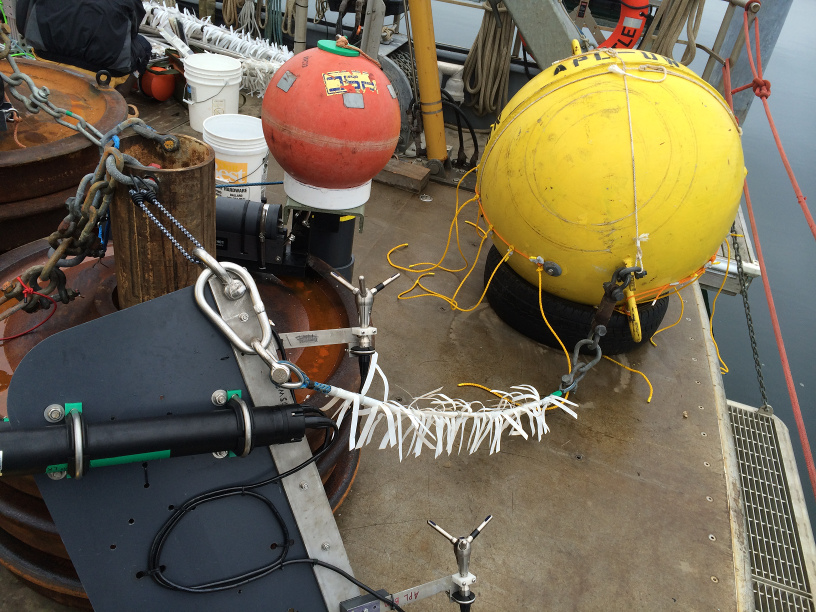
\includegraphics[width=2.6in]{TTM_image01}  
  \caption{TTM components on the deck of the R/V Jack Robertson. The TTM includes two ADVs, with pressure-cases mounted on opposite sides of the fin. The anchor stack includes a pop-up buoy for retrieval. }
  \label{fig:ttm:photo}
\end{figure}

\subsubsection{StableMoor}

The second mooring system was a cylindrical syntactic foam buoy (manufacturer: Deep Water Buoyancy) that was anchored to a clump weight that weighed 2700 lbs (Figure \ref{fig:SM}). The buoy is 3.5 m long and 0.45 m in diameter with a tail ring that is 0.76 m in diameter. The buoy was deployed from 11:21 on May 11, 2016 to 12:00 on May 12, 2016 at 48.15277 north, 122.68623 west.

The StableMoor platform has two primary advantages compared to the TTM. First, it is significantly more massive and hydro-dynamically stable than the TTM, which reduces the frequency of motions of the platform. The other major advantage of the StableMoor platform is that it is capable of supporting an acoustic Doppler profiler that provides an independent measure of the platform's translational motion by bottom-tracking. The disadvantages of the Stable Moor is that its size introduces new challenges in deployment and recovery, and it is significantly more expensive than the TTM system.

The StableMoor weighs 295 kg in air, and has a buoyancy of 185 kg in water. An ADV head was positioned 0.1 m in front of the buoy nose.  The buoy was equipped with a 1200 kHz RDI workhorse sentinel acoustic Doppler profiler that was pointed downward and configured to measure water velocity below the platform in 12 1-meter bins and measure buoy motion (`bottom tracking'), all at a 1 Hz sample rate. The bottom track velocity provides an independent measure of platform motion that aids in correcting velocity measurements for mooring motion.

The buoy platform was ballasted to pitch upward a few degrees in zero-flow to avoid `flying downward'. In the presence of an oncoming current the tail fins help to orient it into the flow. The anchor for this buoy is similar to that of the TTM, including an acoustic release so the mooring and anchor can be recovered separately. Additional details, photos, and schematic diagrams of both mooring systems are available in \cite{Harding_MotionPaper}.

\begin{figure}[t]
  \centering
  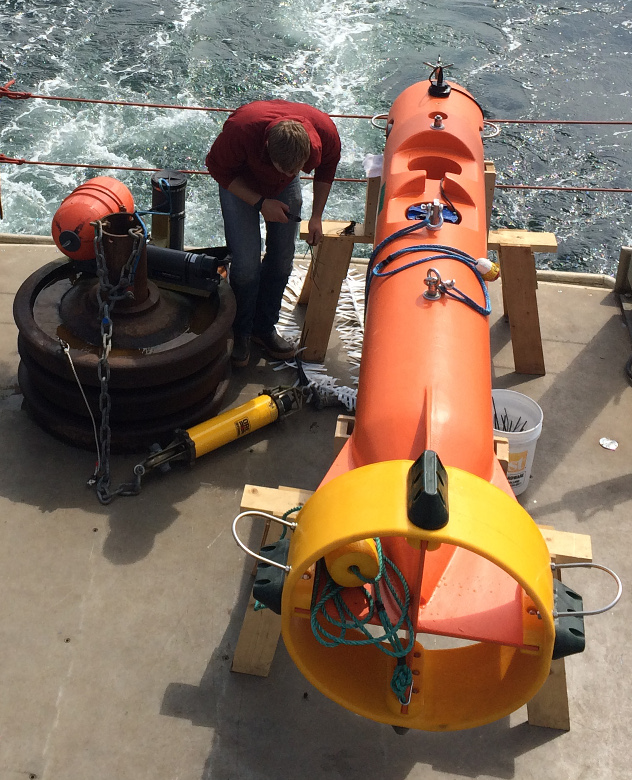
\includegraphics[width=2.6in]{SM_ondeck01}
  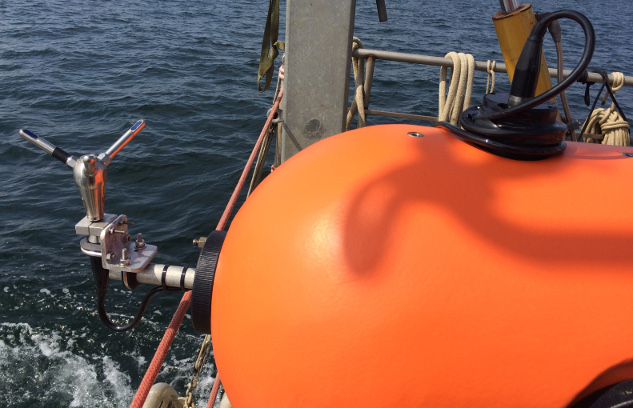
\includegraphics[width=2.6in]{SM_NoseMode01}
  \caption{Alex DeKlerk checks to ensure that the StableMoor buoy is properly fastened to its anchor; the RDI workhorse ADCP can be seen in the rear instrument bay (top). A bridle is draped across the top of the buoy for deployment and recovery, and a small marker buoy fastened to the tail is useful during recovery.  A close-up of the StableMoor nose shows the ADV head and the top of its pressure case (bottom). }
  \label{fig:SM}
\end{figure}


\subsection{Principal-axes coordinate system and turbulence averaging}

Unless stated otherwise, vector quantities in this work are in a fixed `principal-axes' coordinate system that is aligned with the bi-directional tidal flow: positive $u$ is in the direction of ebb (310$^\circ$ True), positive $w$ is vertically upward, and $v$ is the cross-stream component in a right-handed coordinate system. The full velocity vector, $\vec{\tilde{u}} = (\tilde{u}, \tilde{v}, \tilde{w})$, is separated into a mean and turbulent component as $\vec{\tilde{u}} = \vec{\bar{u}} + \vec{u}$, where the over-bar denotes a 5 minute average. Throughout this work we use $\bar{U} = (\bar{u}^2+\bar{v}^2)^{1/2}$ to denote the horizontal velocity magnitude.

All spectra, $\spec{x}(f)=|\fourier{x(t)}|^2$, and cross-spectra, $\cspec{x}{y}(f)=\mathrm{real}(\fourier{x(t)}\fourier{y(t)})$, are computed using NumPY fast Fourier transform routines \cite[]{Walt++2011}. Here, $\fourier{x(t)}$ denotes the fast Fourier transform of a signal $x(t)$.  Time series' are linearly detrended and Hanning windowed prior to computing $\fourier\{x\}$ to reduce spectral reddening.  Throughout the remainder of this work the dependence of $S$ and $C$ on $f$ is implied (e.g. $\spec{x}(f)$ is hereafter $\spec{x}$), and all other variables are functions of $t$. Spectra and cross-spectra are normalized to preserve variance: $\int \spec{u}\mathrm{d}f = \overline{u^2}$, and  $\int \cspec{u}{v}\mathrm{d}f = \overline{uv}$.

Turbulence dissipation rates are computed as,
\begin{align}
  \epsilon = \frac{1}{\bar{U}}\left(\alpha\left\langle(\spec{u}+\spec{v}+\spec{w})f^{5/3}\right\rangle_{f_{IS}}\right)^{3/2}
\end{align}
Where  $\alpha=0.5$, and $\langle\rangle_{f_{IS}}$ denotes an average over the inertial-subrange of the velocity spectra and where the signal-to-noise ratio is small \cite[]{Lumley+Terray1983,Sreenivasan1995}. Throughout this work we take this average from 0.3 to 1 Hz for the $u$ and $v$ components, and 0.3 to 3 Hz for the $w$ component.



%%% Local Variables:
%%% mode: latex
%%% TeX-master: "Kilcher_etal_IMU-ADV"
%%% End:
